\documentclass[eikonal.tex]{subfiles}

\begin{document}
  
\section{Implementation of the ordered line integral
  method}\label{sec:implementation}

\begin{figure}[t]
  \centering
  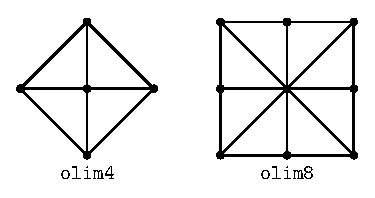
\includegraphics{neighborhood-2d.eps}
  \caption{Neighborhoods of the two-dimensional ordered line integral
    methods \texttt{olim4} and
    \texttt{olim8}.}\label{fig:neighborhood-2d}
\end{figure}

\begin{figure}[t]
  \centering
  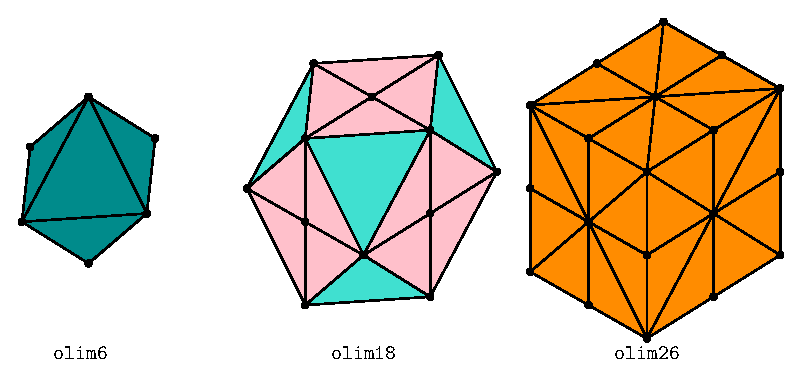
\includegraphics{neighborhood-3d.eps}
  \caption{Neighborhoods of the 3D ordered line integral methods
    \texttt{olim6}, \texttt{olim18}, and
    \texttt{olim26}.}\label{fig:neighborhood-3d}
\end{figure}

In this section, we describe how to implement \cref{enum:update-U} of
\cref{alg:dijkstra-like} efficiently. The emphasis of this section is
the solver in 3D, since implementation in 2D is straightforward, and
there are fewer performance considerations. The main issue is how to
quickly enumerate tetrahedron updates while avoiding unnecessary ones,
of which there are potentially many. We start by showing how we
enumerate tetrahedra in a way that lets us avoid redundant overlapping
tetrahedron updates. We then discuss a projected Newton's method for
solving \cref{eq:constrained-minimization}. These first two sections
can be combined into a ``top-down'' hierarchical update algorithm. In
the following section, we apply KKT theory to avoid unnecessary
simplex updates by determining when they possess interior point
solutions, which leads to a ``bottom-up'' hierarchical update
algorithm. Following this, we outline and categorize the specific
choices of parameters for these algorithms that we use in our
numerical tests. Finally, we describe how our algorithm can be applied
to the additively factored eikonal equation.

\begin{figure}[t]
  \centering
  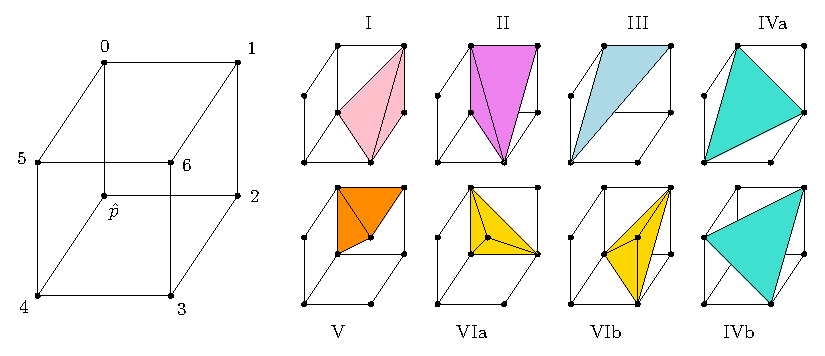
\includegraphics{simplex-groups.eps}
  \caption{Numbering scheme for an update octant. In this diagram,
    $\hat{p}$ is being updated. The diagonally opposite node is the
    sixth (last) node, with the other six nodes numbered 0--5
    cyclically.}\label{fig:octant-numbering}
\end{figure}

\begin{figure}[t]
  \centering
  {
    \footnotesize
    \begin{tabular}{c|cccccc|cccccc|cccccc|cc}
      0 & $\groupmarker$ & & & & $\groupmarker$ & $\groupmarker$ & $\groupmarker$ & & & $\groupmarker$ & & $\groupmarker$ & $\groupmarker$ & & $\groupmarker$ & & & $\groupmarker$ & $\groupmarker$ & \\
      1 & $\groupmarker$ & $\groupmarker$ & & & & $\groupmarker$ & $\groupmarker$ & $\groupmarker$ & & & $\groupmarker$ & & $\groupmarker$ & $\groupmarker$ & & $\groupmarker$ & & & & $\groupmarker$ \\
      2 & $\groupmarker$ & $\groupmarker$ & $\groupmarker$ & & & & & $\groupmarker$ & $\groupmarker$ & & & $\groupmarker$ & & $\groupmarker$ & $\groupmarker$ & & $\groupmarker$ & & $\groupmarker$ & \\
      3 & & $\groupmarker$ & $\groupmarker$ & $\groupmarker$ & & & $\groupmarker$ & & $\groupmarker$ & $\groupmarker$ & & & & & $\groupmarker$ & $\groupmarker$ & & $\groupmarker$ & & $\groupmarker$ \\
      4 & & & $\groupmarker$ & $\groupmarker$ & $\groupmarker$ & & & $\groupmarker$ & & $\groupmarker$ & $\groupmarker$ & & $\groupmarker$ & & & $\groupmarker$ & $\groupmarker$ & & $\groupmarker$ & \\
      5 & & & & $\groupmarker$ & $\groupmarker$ & $\groupmarker$ & & & $\groupmarker$ & & $\groupmarker$ & $\groupmarker$ & & $\groupmarker$ & & & $\groupmarker$ & $\groupmarker$ & & $\groupmarker$ \\
      \multicolumn{1}{c}{} & \multicolumn{6}{c}{I} & \multicolumn{6}{c}{II} & \multicolumn{6}{c}{III} & \multicolumn{2}{c}{IV}
    \end{tabular}%
    \vspace{1em}
    \begin{tabular}{c|cccccc|cccccc|ccc}
      0 & $\groupmarker$ & & & & & $\groupmarker$ & $\groupmarker$ & & & & $\groupmarker$ & & $\groupmarker$ & & \\
      1 & $\groupmarker$ & $\groupmarker$ & & & & & & $\groupmarker$ & & & & $\groupmarker$ & & $\groupmarker$ & \\
      2 & & $\groupmarker$ & $\groupmarker$ & & & & $\groupmarker$ & & $\groupmarker$ & & & & & & $\groupmarker$ \\
      3 & & & $\groupmarker$ & $\groupmarker$ & & & & $\groupmarker$ & & $\groupmarker$ & & & $\groupmarker$ & & \\
      4 & & & & $\groupmarker$ & $\groupmarker$ & & & & $\groupmarker$ & & $\groupmarker$ & & & $\groupmarker$ & \\
      5 & & & & & $\groupmarker$ & $\groupmarker$ & & & & $\groupmarker$ & & $\groupmarker$ & & & $\groupmarker$ \\
      6 & $\groupmarker$ & $\groupmarker$ & $\groupmarker$ & $\groupmarker$ & $\groupmarker$ & $\groupmarker$ & $\groupmarker$ & $\groupmarker$ & $\groupmarker$ & $\groupmarker$ & $\groupmarker$ & $\groupmarker$ & $\groupmarker$ & $\groupmarker$ & $\groupmarker$ \\
      \multicolumn{1}{c}{} & \multicolumn{6}{c}{V} & \multicolumn{6}{c}{VI} & \multicolumn{3}{c}{VII}
    \end{tabular}%
    \vspace{-0.5em}
  }
  \caption{These tables should be scanned columnwise: each column of
    dots indicates a different tetrahedron. Note that the tetrahedra
    (0, 1, 2), (2, 3, 4), and (4, 5, 0) in group I are degenerate and
    can be omitted. The tetrahedra in group VII are all degenerate and
    can do not form a useful group.}\label{fig:tetrahedra-groups}
  \vspace{1em}
\end{figure}

\subsection{Simplex selection}

Computing $U(\hat{p})$ consists of determining a set of possible
directions for the first arrival characteristic of \cref{eq:eikonal},
and then solving a collection of optimization problems to locate
it. In 2D, we consider two types of neighborhoods: those for which
$\hat{p} - p$ has at most one nonzero component, and those with at
most two nonzero components (recalling that we always assume
$\norm{p}_\infty \leq 1$ for $p \in \mathbb{Z}^n$). The former is the
$\ell_1$ neighborhood of $\hat{p}$, the latter is the $\ell_\infty$
neighborhood. We also consider the $\ell_1$ and $\ell_\infty$
neighborhoods in 3D, which correspond to 6-point and 26-point
neighborhoods, respectively; there is also an 18-point neighborhood,
consisting of neighbors with two nonzero components. A simple way of
characterizing these neighborhoods is in terms of the ``zero norm'' or
cardinality, $\norm{p}_0$, which is just the number of nonzero
components of a vector. Then, in 2D, we consider neighborhoods where
$\norm{p}_0 \leq k$, where $k = 1, 2$; in 3D, $k = 1, 2, 3$. More
generally, in $n$ dimensions, we could consider neighborhoods where
$1 \leq k \leq n$.

With $\neib(\hat{p})$ so defined, we need to determine which simplexes
are candidates for optimization. With only $p_i$.\texttt{state} as a
criterion, we end up traversing a larger number of simplexes than is
strictly necessary for consistency. In 3D, we discretize the surface
of the convex hull of $\neib(\hat{p})$ into triangles and let the set
of admissible triangles and tetrahedra be the set of convex hulls of
the lines and triangles joining this discretized surfaces with
$\hat{p}$. For the 6-point, 18-point, and 26-point neighborhoods,
these surfaces are an octahedron, cuboctahedron, and cube,
respectively.

Another approach is to assume that the simplexes within each orthant
are the same. Then, we can restrict our attention to a single orthant
and determine the admissible simplexes by selecting vertices. We would
like these simplexes to be symmetric about the diagonal of the orthant
so that our update is isotropic. Following this idea, we decompose an
octant into groups of tetrahedra in
\cref{fig:octant-numbering,fig:olim18-tetrahedra,fig:olim26-tetrahedra}. The
groups are defined in
\cref{fig:olim18-tetrahedra,fig:olim26-tetrahedra}, while
\cref{fig:octant-numbering} provides a visual overview. We partially
sort the vertices of octant by degree, allowing us to easily separate
our groups into groups which features in the 6-point, 18-point, or
26-point neighborhoods. In our implementation, separating the
simplexes into groups allows us to generate sections of straight-line
code which can be conditionally enabled at compile time so that we
only traverse the specified simplexes.

\subsection{Update gaps for tetrahedron groups}

If we apply \cref{thm:causality} to the tetrahedron groups enumerated
in
\cref{fig:octant-numbering,fig:olim18-tetrahedra,fig:olim26-tetrahedra},
we find that the groups have the following update gaps (ignoring the
$s^\theta h$ factor):
\vspace{0.5em}
\begin{center}
  \begin{tabular}{lc|lc|lc|lc}
    Group I & $1/\sqrt{2}$ & Group II & $1/\sqrt{2}$ & Group III & $1/\sqrt{2}$ & Group IVa & 0 \\
    \midrule
    Group V & $1/\sqrt{3}$ & Group VIa & 0 & Group VIb & $\boldsymbol{2/\sqrt{3}}$ & Group IVb & $1/\sqrt{2}$
  \end{tabular}
\end{center}
\vspace{0.5em} The idea of the update gap is first explored in
Tsitsiklis's original paper~\cite{tsitsiklis1995efficient}. In this
work, the fact that Group IVa has no update gap and that the update
gap of Group V is $1/\sqrt{3}$ is noted and an $O(N)$ algorithm based
on Dial's algorithm is presented using Group V for the update
tetrahedra. This same observation is made in a more recent paper
explicitly detailing a method based on Dial's
algorithm~\cite{kim2001calo}. A method based on a combination of
tetrahedra groups will have as its update gap the minima of each of
the individual groups' update gaps. Since a combination of Groups I
and VIb should provide similar performance characteristics as a method
based on Group V, we can see that using these groups would lead to a
larger update gap: $1/\sqrt{2}$ instead of $1/\sqrt{3}$. This should
have a positive impact on performance and will be investigated in a
future work.

\subsection[Optimization algorithms]{Minimization algorithms}

In this section, we describe two algorithms for solving the
constrained minimization problem
\cref{eq:constrained-minimization}. To compute $U(\hat{p})$ in
\cref{alg:dijkstra-like}'s \cref{enum:update-U}, multiple instances of
\cref{eq:constrained-minimization} with overlapping boundaries must be
solved. The fact that the boundaries of their domains may overlap
leads to different approaches to solving all instances of
\cref{eq:constrained-minimization} in tandem. This is discussed in the
next section. The difference lies in whether we order the updates in
increasing or decreasing order by the dimension $d$. In the former
case (``bottom-up''), we use KKT theory to apply information about
lower dimensional updates to avoid higher dimensional updates; in the
latter case (``top-down''), we use our grouping of simplexes to avoid
redundantly computing boundary updates.

For the following two algorithms, we assume that $F_i$ is strictly
convex. By \cref{lemma:dPt-cprojp-dP-pd,lemma:F-strictly-convex}, this
is always the case for $F_0$ and holds for $F_1$ if $h$ is small
enough ($h < \hthresh$).

We first consider the bottom-up minimization algorithm. Although
\cref{eq:constrained-minimization} is a constrained problem, we can
take advantage of \cref{theorem:mp0-newton,thm:f0-exact} to instead
solve an unconstrained problem by first computing $\lambda_0^*$ from
\cref{thm:f0-exact} and then letting $\lambda_0 = \lambda_0^*$ be the
initial iterate of an unconstrained Newton iteration minimizing
$F_1$. \Cref{theorem:mp0-newton,thm:f0-exact} give us conditions for
determing when this be done: in particular, we first check if
$\norm{R^{-\top} \delU} < s^\theta h$, then check if $\lambda_1^*$
is inside $\Delta^n$. If this isn't the case, we can always default to
a constrained solver (described below). To check if
$\lambda_1^* \in \Delta^n$, we can use the proof of
\cref{theorem:mp0-newton}, which states that $\lambda_1^*$ lies in the
closed ball $B_r(\lambda_0^*)$, where:
\begin{equation}
  r \leq R = \frac{\alpha}{1 - \alpha/2}, \mbox{ and } \alpha = \norm{\nabla^2 F_1(\lambda_0^*)^{-1} \nabla F_1(\lambda_0^*)}.
\end{equation}
Checking whether $\lambda_1^*$ is in $\Delta^n$ can then be done by
checking if $B_R(\lambda_0^*)$ is contained in $\Delta^n$, which is
straightforward and inexpensive.

\begin{algorithm}[H]
  \caption{Newton's method with warm start for solving
    \cref{eq:constrained-minimization} with
    $F_i = F_1$.}\label{alg:warm-start-newton}
  \begin{enumerate}[nolistsep]
  \item Compute the reduced QR decomposition $\delP = QR$. Since we
    only deal with a small, fixed number of simplexes, all QR
    decompositions can be procomputed.
  \item Let $\lambda_0 = \lambda^*$ in \cref{eq:f0-exact-lambda}.
  \item If $B_R(\lambda_0) \subseteq \Delta^n$, then:
    \begin{enumerate}[nolistsep]
    \item For $k = 1, 2, \hdots$ until convergence:
      \begin{enumerate}
      \item Set
        $\lambda_k = \lambda_{k-1} - \nabla^2
        F_1(\lambda_{k-1})^{-1} \nabla
        F_1(\lambda_{k-1})$.
      \end{enumerate}
    \item Evaluate $\hat{U}$ using the last $\lambda_k$ iterate.
    \end{enumerate}
  \item Otherwise, run \cref{alg:proj-newton}.
  \end{enumerate}
\end{algorithm}

Our second algorithm is a projected Newton's method, which is
standard~\cite{bertsekas1999nonlinear,nocedal2006numerical}. We use
this algorithm for the top-down strategy. Minimizing $F_i(\lambda)$,
if we let $\lambda_k$ ($k = 0, 1, \hdots$) be a sequence of iterates
and $\lambda_{k+1} = \lambda_k + \dellam_k$, we can Taylor
expand:
\begin{equation}
  F_i(\lambda_k + \dellam_k) = F_i(\lambda_k) + \nabla F_i(\lambda_k)^\top \dellam_k + \frac{1}{2} \dellam_k^\top \nabla^2 F_i(\lambda_k) \dellam_k + O(\norm{\dellam_k}^3).
\end{equation}
A common method of minimizing a nonlinear function is to minimize a
sequence of local quadratic approximations, known as a sequential
quadratic program (SQP). If our goal is to minimize
$F_i(\lambda_{k+1})$, we then find an approximate optimum by solving:
\begin{equation}\label{eq:local-quadratic-minimization}
  \begin{split}
    \min_{\lambda} &\qquad \frac{1}{2} \lambda^\top \nabla^2 F_i(\lambda_k) \lambda + \nabla F_i(\lambda_k)^\top \lambda \\
    \text{subject to} &\qquad \lambda \in \Delta^d.
  \end{split}
\end{equation}
\Cref{eq:local-quadratic-minimization} is an inequality constrained
quadratic program (IQP) which can be solved using the active set
method, which is similar to the simplex algorithm for solving linear
programs~\cite{nocedal2006numerical}. Briefly: a Newton step is
attempted---if the step collides with a constraint, the constraints
are cycled until a minimum is found. In our implementation, we warm
start our active set method with the current iterate to accelerate
it. One thing to note is that the constraints encapsulated by
$\lambda \in \Delta^d$ can be written in matrix form (e.g., for
$d = n$) as:
\begin{equation}
  \label{eq:matrix-ineq}
  A \lambda \geq b, \qquad \text{where} \qquad A = \begin{bmatrix}
    -\m{1}_{1 \times n} \\ I_n
  \end{bmatrix}, \qquad b = \begin{bmatrix} -1 \\ \m{0}_{n \times 1} \end{bmatrix}.
\end{equation}
The simplicity of \cref{eq:matrix-ineq} makes the implementation of
the active set method for solving
\cref{eq:local-quadratic-minimization} simple and efficient. For more
details, the source of our implementation can be
consulted~\cite{sfp-umiacs-homepage}. Details such as initializing the
active set with a warm start, which are used in our implementation,
can be found in standard references~\cite{nocedal2006numerical}.

\begin{algorithm}[H]
  \caption{Projected Newton's method for solving
    \cref{eq:constrained-minimization} with
    $F_i = F_1$.}\label{alg:proj-newton}
  \begin{enumerate}[nolistsep]
  \item Initialize $\lambda_0$. We take $\lambda_0$ to be the centroid
    of $\Delta^n$, or $\lambda_0^*$ if it exists.
  \item For $k = 1, 2, \hdots$ until convergence:
    \begin{enumerate}
    \item Set $H_k = \nabla^2 F_1(\lambda_k)$.
    \item Perturb $H_k$ by a small multiple of $I$ if $H_k$ isn't
      positive definite (optional, depending on $h$).
    \item Set $g_k = \nabla F_1(\lambda_k) - H_k \lambda_k$.
    \item Compute $p_k = \dellam_k$ by solving
      $p_k = \argmin_{Ap \geq b - A\lambda_k} p^\top H_k p + g_k^\top
      p$ using the active set method.
    \item Compute a step size $\gamma_k$ using line search.
    \item Let $\lambda_{k + 1} = \lambda_k + \gamma_k p_k$.
    \end{enumerate}
  \item Compute $\hat{U}$ from the final $\lambda_k$.
  \end{enumerate}
\end{algorithm}

The foregoing algorithm can be initialized with its initial iterate
set to $\lambda_0^*$. However, we note that in practice---especially
as $h \to 0$---this algorithm only requires around 3--5 iterations to
converge, and frequently converges in one iteration, even if
$\lambda_0$ is initialized to the centroid of $\Delta^n$. This is
optimal, given that Newton's method converges quadratically, and that
$\norm{\dellam_k} \leq \sqrt{d}$ since our iterates are
constrained to lie in $\Delta^n$.

\begin{figure}[t]
  \centering
  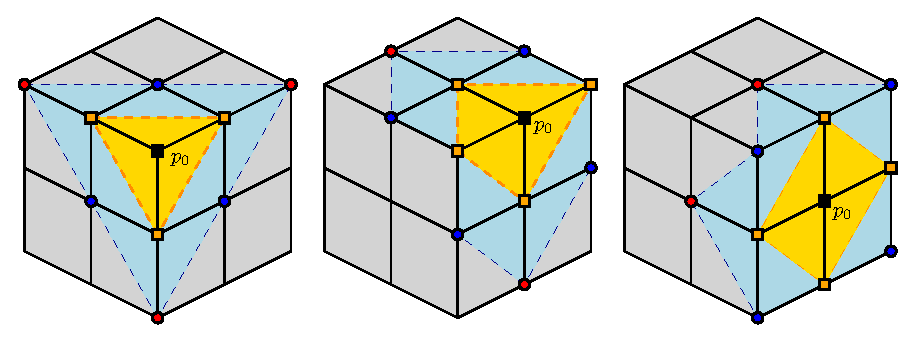
\includegraphics[width=0.85\linewidth]{hu-neighborhoods.eps}
  \caption{The three types of neighborhoods for
    \cref{alg:bottom-up}. The yellow and blue regions indicate where
    triangle and tetrahedron updates may be performed,
    respectively. For instance, once $p_0$ is determined, candiates
    for $p_1$ consist of the yellow nodes: triangle updates involving
    these candidates and $p_0$ will be performed. Once the minimizing
    triangle update is computed, tetrahedron updates corresponding to
    the neighboring blue nodes will be computed, as well---for each of
    the three neighborhoods, this means that at most two tetrahedron
    updates will be performed per round of updates. Note that the
    updates performed correspond roughly to a combination of groups I,
    V, VIa, and VIb.}\label{fig:hu-neighborhoods}
\end{figure}

\subsection[Update algorithms]{Hierarchical update algorithms}

We now describe our bottom-up and top-down algorithms for updating a
node, starting with the bottom-up approach. For any dimension $n$, we
start by computing the minimal line update, letting the corresponding
node be denoted by $p_0$. We then evaluate each triangle update whose
base contains $p_0$, by searching through other nearby (within a
distance of $h$) nodes---we let the node corresponding to the minimum
triangle update be denoted $p_1$. Likewise for each tetrahedron, and
so on. The specific way that we do this, which we refer to as
\texttt{olimhu}, is shown in \cref{fig:hu-neighborhoods}. Once $p_0$
is found, the yellow nodes in \cref{fig:hu-neighborhoods} show the
location of candidates for $p_1$; likewise, the blue nodes show where
$p_2$ may lie. In addition, we require that $p_2$ be within a distance
of $h \sqrt{2}$ of both $p_0$ and $p_1$, so that at most two
tetrahedron updates are done each time a node is updated. This is
beneficial, since this implies that at most $2N$ tetrahedron updates
are done when solving \cref{eq:eikonal}. This approach can be easily
generalized to higher dimensions. We note here that the nascent idea
that led to this algorithm was first developed to accelerate a
Dijkstra-like solver used to compute quasipotentials of nongradient
stochastic differential equations in 2D~\cite{dahiya2017ordered}, and
a similar idea is explored in~\cite{yang2018computing}.

A key benefit of this approach is that it streamlines the use of
Karush-Kuhn-Tucker (KKT) theory~\cite{nocedal2006numerical} for
skipping higher degree updates. We describe this now. First, we define
the Lagrange function of \cref{eq:constrained-minimization}:
\begin{equation}
  L_i(\lambda, \mu) = F_i(\lambda) + {(A\lambda - b)}^\top \mu.
\end{equation}
Since \cref{eq:constrained-minimization} only has linear inequality
constraints, and since we assume that $F_i$ is strictly convex
according to \cref{lemma:dPt-cprojp-dP-pd,lemma:F-strictly-convex},
checking the KKT conditions for \cref{eq:constrained-minimization} is
straightforward. If $(\lambda^*, \mu^*)$ satisfy:
\begin{equation}
  \label{eq:kkt}
  \begin{split}
    \nabla_\lambda L_i(\lambda^*, \mu^*) &= 0, \\
    A\lambda^* &\geq b, \\
    \mu^* &\geq 0, \\
    (A\lambda^* - b)^\top \mu^* &= 0,
  \end{split}
\end{equation}
then $\lambda^*$ is a global minimizer over $\Delta^n$, where $A$ and
$b$ are defined in \cref{eq:matrix-ineq}. The first two conditions
tell us that the iterate is stationary and that it lies in the
constraint set. For the second two conditions, computing $\mu^*$ is
easily done. Altogether, \cref{eq:kkt} gives us a simple and cheap
test that allows us to check whether a simplex update provides
additional information beyond what would be obtained by solving
\cref{eq:constrained-minimization} on each of its boundary simplexes.

For convenience, we describe how to compute $\mu^*$ here. Assume the
first two conditions of \cref{eq:kkt} hold for $\lambda \in \Delta^n$,
let $I$ be the set of active constraints:
\begin{equation}
  I = \set{i : (A\lambda)_i = b_i, \hspace{0.25em} 0 \leq i < n},
\end{equation}
and let $A_I$ be a matrix consisting of the columns of $A$ indexed by
$I$, and let $\lambda_I$ and $b_I$ be subvectors of $\lambda$ and $b$
indexed by $I$. Consider the equality-constrained quadratic program:
\begin{equation}
  \label{eq:active-set-EQP}
  \begin{split}
    \min_{\dellam} &\qquad \frac{1}{2} \dellam^\top \nabla^2 F_i^\theta (\lambda) \dellam + \nabla F_i^\theta(\lambda)^\top \dellam \\
    \text{subject to} &\qquad A_I \dellam = b_I - A_I \lambda,
  \end{split}
\end{equation}
which determines a descent step $\dellam^*$. The KKT system
corresponding to \cref{eq:active-set-EQP} is:
\begin{equation}
  \begin{bmatrix}
    \nabla^2 F_i (\lambda) & -A_I^\top \\
    A_I & 0
  \end{bmatrix} \begin{bmatrix}
    \dellam^* \\ \mu^*
  \end{bmatrix} = \begin{bmatrix}
    -\nabla F_i(\lambda) \\ 0
  \end{bmatrix}.
\end{equation}
Solving this system, the vector of Lagrange multipliers can be
computed from:
\begin{equation}\label{eq:mu-star}
  \mu^* = {(A_I \nabla^2 F_i(\lambda)^{-1} A_I^\top)}^{-1} A_I \nabla^2 F_i(\lambda)^{-1} \nabla F(\lambda).
\end{equation}
If $\mu^* \geq 0$, then $\mu^*$ corresponds to the a global
constrained optimum over $\Delta^n$. Although \cref{eq:mu-star}
appears moderately complicated, the simple form of $A$, defined in
\cref{eq:matrix-ineq}, causes \cref{eq:mu-star} to simplify
nicely. For instance, for a triangle update, we can equivalently check
the sign of the derivative of $F_i$ at either end of the interval
$\Delta^1 = [0, 1]$. The checks for tetrahedron updates are not much
more complicated.

To determine whether a simplex contains an interior point solution, we
need to check $\mu^*$ corresponding to the optimum $\lambda^*$ on each
of its boundary simplexes. Progressing from lower to higher
dimensional updates, we visit parts of the boundaries first. Caching
each $\lambda^*$ as we go, we can rule out more expensive updates
before we need to do them.

\begin{algorithm}[H]
  \caption{A bottom-up hierarchical algorithm for computing
    $U(\hat{p})$ (\cref{enum:update-U} of
    \cref{alg:dijkstra-like}).}\label{alg:bottom-up}
  \begin{enumerate}[nolistsep]
  \item Set $\hat{U} \gets \infty$.
  \item Find $p_0 \in \neib(\hat{p})$ such that $p_0$\texttt{.state}
    $=$ \texttt{valid} with the minimum update value for $d = 0$;,
    i.e., the one-point update.
  \item For $i = 1, \hdots, n - 1$:
    \begin{enumerate}
    \item For each \texttt{valid} $p_i$ chosen hierarchically (see
      \cref{fig:hu-neighborhoods}):\label{item:bottom-up-for}
      \begin{enumerate}
      \item For each choice of $i - 1$ nodes from $p_0, \hdots, p_i$,
        compute $\mu^*$ corresponding to $\lambda^*$. If $\lambda^*$
        is a global constrained optimum, continue to the next
        iteration of \cref{item:bottom-up-for}.
      \item Do the update corresponding to $p_0, \hdots, p_{i}$ using
        \cref{alg:warm-start-newton}, update $\hat{U}$, and cache
        $\lambda^*$ if $i < n - 1$.
      \end{enumerate}
    \end{enumerate}
  \end{enumerate}
\end{algorithm}

Now we describe the top-down approach. As an algorithm, it is
comparatively simpler. Let $\calC_d$ be the set of $d$-dimensional
update simplexes for $\hat{p}$ containing only \texttt{valid}
vertices. Since \cref{alg:proj-newton} computes the constrained global
optimum over an update simplex, after running it, we can rule out any
incident update simplexes on its boundary. Starting from $d = n - 1$,
we can progressively rule out large numbers of incident subsimplexes
and substantially reduce the number of updates that need to be done to
compute $\hat{U}$. We note that at each step, we remove \emph{all}
lower-dimensional updates---e.g., after computing a tetrahedron
update, we eliminate all incident triangle and line updates.
\begin{algorithm}[H]
  \caption{A top-down hierarchical algorithm for computing
    $U(\hat{p})$ (\cref{enum:update-U} of
    \cref{alg:dijkstra-like}).}\label{alg:top-down}
  \begin{enumerate}[nolistsep]
  \item Set $\hat{U} \gets \infty$.
  \item For $d = n - 1$ down to $0$:
    \begin{enumerate}
    \item For each $(p_0, \hdots, p_{d}) \in \calC_d$:
      \begin{enumerate}
      \item Compute $U$ for the update simplex
        $(p_0, \hdots, p_{d})$ using \cref{alg:proj-newton}.
      \item Set $\hat{U} = \min(\hat{U}, U)$.
      \item Remove each incident boundary simplex from
        $\calC_1, \hdots, \calC_{d-1}$.
      \end{enumerate}
    \end{enumerate}
  \end{enumerate}
\end{algorithm}
\noindent If we try to skip updates using KKT theory in
\cref{alg:top-down}, we end up recovering a recursive version of
\cref{alg:bottom-up}. This would require a more complicated data
structure to implement, and seems unlikely to perform favorably
compared to \cref{alg:bottom-up}.

\begin{figure}
  \centering
  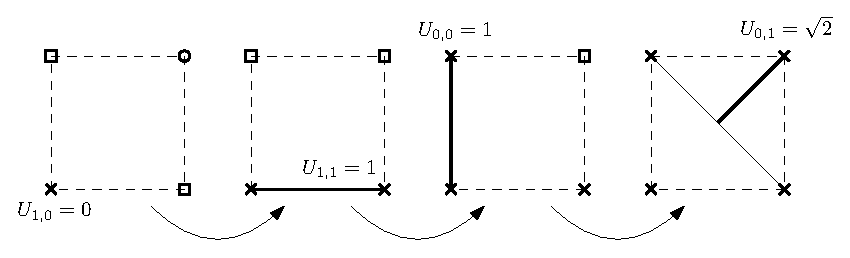
\includegraphics{factoring-example.eps}
  \caption{Factoring in action. This figure shows three steps of a
    factored \texttt{olim4rhr} (or, equivalently, the four-point fast
    marching method with factoring~\cite{qi2018corner}). Ordered
    clockwise from the top left, the nodes are
    $p_{0, 0}, p_{0, 1}, p_{1, 1}$, and $p_{1, 0}$, with $h = 1$ (so
    we assume our domain is identified with $\mathbb{Z}^2$). We assume
    a constant slowness function: $s \equiv 1$. Initially,
    $p^\circ = p_{1, 0}$ is the only node in \texttt{bd} and is
    factored. The first two steps proceed exactly the same as for the
    unfactored method, since the steps between the source nodes and
    the updated nodes lie along characteristics of the solution,
    $u$. In the third step, the unfactored method would set
    $U_{0,1} \gets 1 + \nicefrac{\sqrt{2}}{2}$. For the factored
    method, since $\tau_{0,1} = 1 - 1 = 0 = \tau_{1,0}$, we find that
    $U_{0,1} \gets 0 + s^\circ l^\circ_{\nicefrac{1}{2}} + s^\theta h
    l_{\nicefrac{1}{2}} = \nicefrac{\sqrt{2}}{2} +
    \nicefrac{\sqrt{2}}{2} = \sqrt{2}$.}\label{fig:factoring-example}
\end{figure}

\subsection{Algorithms used in the numerical
  tests}\label{ssec:specific-algorithms}

To test our family of algorithms, we focus on a representative
cross-section of algorithms and evaluate them numerically in
\cref{sec:numerical-results}. For each quadrature rule described in
\cref{ssec:quadrature} (\texttt{mp0}, \texttt{mp1}, or \texttt{rhr}),
we have two 2D algorithms, \texttt{olim4} and \texttt{olim8},
corresponding to 4- and 8-point stencils, respectively. Since there is
no advantage in 2D, we don't apply the top-down or bottom-up
approaches. In 3D, we have three top-down algorithms: \texttt{olim6}
(group IVa), \texttt{olim18} (groups I, IVa, and IVb), and
\texttt{olim26} (group V). We also test the bottom-up algorithm
\texttt{olimhu} (see \cref{fig:hu-neighborhoods}).

\subsection{Local factoring}

Near rarefaction fans, for example if $D$ is a point source or the
domain contains obstacles with corners, the rate of convergence of the
eikonal equation is diminished. For the eikonal equation with point
source data and constant slowness, this degrades the rate of
convergence to $O(h \log h^{-1})$~\cite{qi2018corner}. Different
factored eikonal equations which treat this problem have been
developed~\cite{fomel2009fast,luo2012fast}. In this section, we show
how the ordered line integral method can be easily adapted to additive
factoring, and provide numerical tests that show that it recovers the
expected linear rate of convergence for factored problems. Our focus
is locally factored point sources, but this approach can be applied to
the globally factored equation and other types of rarefaction fans
occuring at corners or discontinuities~\cite{qi2018corner}.

Let $x^\circ$ be the position of a point source so that
$\boundary = \set{x^\circ}$ and let the grid
$\calG \subseteq \mathbb{Z}^n$ be aligned so that
$p^\circ \in \mathbb{Z}^n$. For a point $p_\lambda$, define
$l^\circ_\lambda = \norm{p_\lambda - p^\circ}$ and let
$s^\circ = s(x^\circ)$. Consider the additive factorization of $U$
around $x^\circ$~\cite{luo2012fast,qi2018corner}:
\begin{align}
  U(x) = T(x) + \tau(x), \qquad \text{where} \qquad T(x) = s^\circ \norm{x - x^\circ},
\end{align}
i.e.\ $u_\lambda = T_\lambda + \tau_\lambda$ where
$T_\lambda = s^\circ h l^\circ_\lambda$. Our original definition of
$F_i^\theta$ was such that $\hat{U} = F_i^\theta(\lambda^*)$. We will
define $G_i^\theta$ analogously. Letting
$\tau_\lambda = \tau_0 + \deltau^\top \lambda$, where $\tau_i$ and
$T_i$ are the values of $\tau$ and $T$ at $p_i$ for each $i$, we
define:
\begin{align}
  \label{eq:Gi}
  G_0(\lambda) = G_0^\theta(\lambda) &= \tau_\lambda + T_\lambda + s^\theta h l_\lambda, \\
  G_1(\lambda) = G_1^\theta(\lambda) &= \tau_\lambda + T_\lambda + s^\theta_\lambda h l_\lambda.
\end{align}
Like with $F_0$ and $F_1$, the only difference between
$G_0$ and $G_1$ is between the terms containing
$s^\theta$ and $s^\theta_\lambda$.

To solve the factored eikonal equation, we choose a factoring radius
$\rfac$, replacing $F_i$ with $G_i$ in
\cref{eq:constrained-minimization} for nodes which lie within a
distance $\rfac$ of $x^\circ$. For constant slowness, the effect of
this is to solve \cref{eq:eikonal} exactly inside of the locally
factored region. For clarity, this is depicted in
\cref{fig:factoring-example}. \Cref{alg:top-down} can be applied to
solve \cref{eq:constrained-minimization} for factored nodes. The
gradient and Hessian of $G_i$ are simple modifications of the gradient
and Hessian for $F_i$.

\begin{lemma}
  The gradient and Hessian of $G_i$ for $i = 0, 1$ are given
  by:
  \begin{align}
    \label{eq:G-grad-hess}
    \nabla G_i(\lambda) &= \nabla F_i(\lambda) - \deltau + \frac{s^\circ h}{l^\circ_\lambda} \delP^\top {(p_\lambda - p^\circ)}, \\
    \nabla^2 G_i(\lambda) &= \nabla^2 F_i(\lambda) + \frac{s^\circ h}{l^\circ_\lambda} \delP^\top \calP^\perp_{p_\lambda - p^\circ} \delP.
  \end{align}
\end{lemma}

\begin{figure}[t]
  \centering
  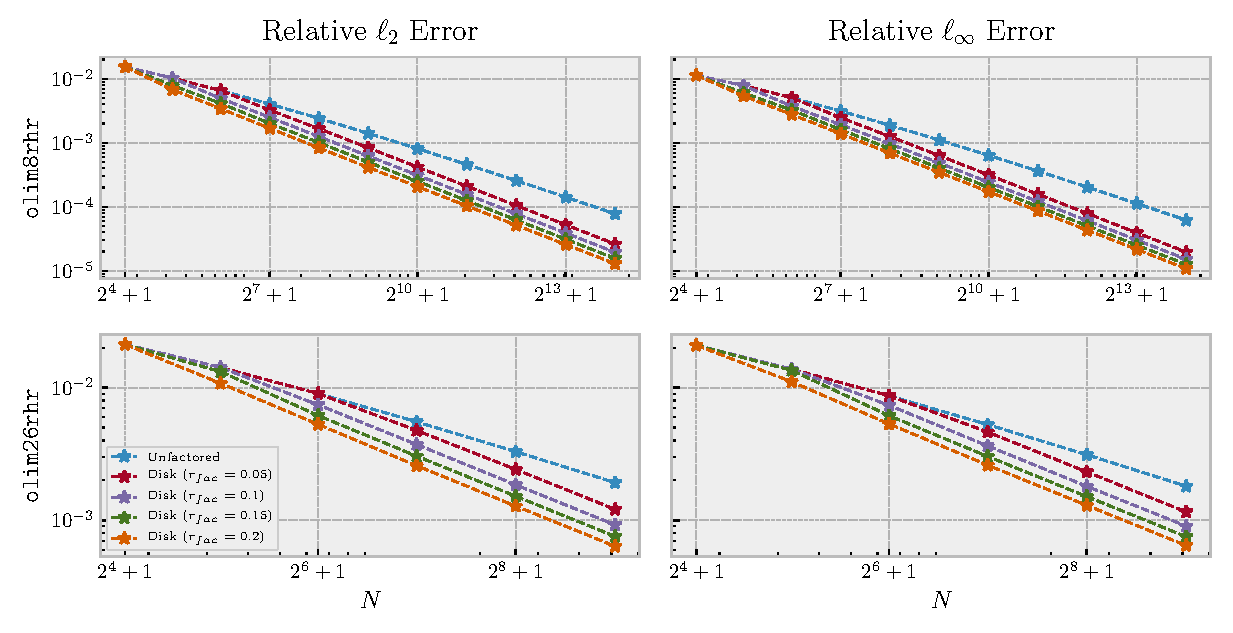
\includegraphics[width=\linewidth]{factoring-error-example.eps}
  \caption{Comparing different ways of selecting factored nodes. For
    the test problem, $\Omega = [-1, 1]^n$, with $n = 2$ (first row)
    and $n = 3$ (second row). The domain is descretized into $N^3$
    nodes, where $N = 2^p + 1$, so that $h = 2/(N - 1)$. The slowness
    function is constant. For the 2D problem, \texttt{olim8rhr} is
    used; \texttt{olim26rhr} is used for the 3D problem. Solutions for
    the unfactored problem are plotted, along with solutions using a
    disk/sphere neighborhood with constant radius given by
    $\rfac = 0.05, 0.1, 0.15, 0.2$. \hl{\textbf{TODO}}: \emph{extend
      max $N$ in plot to $2^{15} + 1$ for 2D and $2^{10} + 1$ for
      3D.}}\label{fig:factoring-error-example}
\end{figure}

Local factoring requires a factored region of constant size with
respect to $h$~\cite{qi2018corner}. For our numerical results
presented in \cref{ssec:point-source-problems}, our domain is
$\Omega = [-1, 1]^n$, for $n = 2, 3$. For these domains, we take
$\rfac = 0.05, 0.1, 0.15, 0.2$. In each case, the linear convergence
is recovered. See~\cref{fig:factoring-error-example}.

\end{document}

%%% Local Variables:
%%% mode: latex
%%% TeX-master: "sisc-eikonal.tex"
%%% End:


